\documentclass[a4paper]{article}

\usepackage{times}
\usepackage{tikz}
\usepackage[margin=0cm]{geometry}
\usepackage{graphicx}
\usepackage{anyfontsize}
\usepackage{fancyhdr}
\usepackage{indentfirst}
\usepackage{amsmath}
\usepackage[spanish]{babel}
\usepackage[utf8]{inputenc}
\usepackage{titlesec}


\author{}
\date{}
\title{}

\begin{document}
\thispagestyle{empty}

\begin{tikzpicture}[remember picture, overlay]
    \pgftransformshift{\pgfpoint{0cm}{0cm}}
    \draw [line width=2pt](1cm,-1cm) -- (1cm,-27.7cm) -- (14cm, -27.7cm) -- (14cm, -1cm) -- (1cm, -1cm);
    \draw[line width=2pt] (15cm, -27.7cm) -- (19cm,-27.7cm) -- (19cm, -1cm) -- (15cm, -1cm) --  (15cm, -27.7cm);
    \node [line width=2pt] at (17cm, -3.5cm) {
\includegraphics[width=3cm]{../utn.png}};
		\node [line width=2pt] at (7.5cm, -7.5cm) {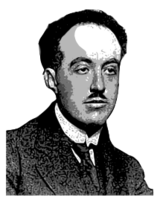
\includegraphics[width=6cm]{../broglie.png}};
    \node at (17cm, -7cm) {\scalebox{5}{\textbf{U}}};
    \node at (17cm, -9cm) {\scalebox{5}{\textbf{T}}};
    \node at (17cm, -11cm) {\scalebox{5}{\textbf{N}}};
    \node at (17cm, -14cm) {\scalebox{5}{\textbf{F}}};
    \node at (17cm, -16cm) {\scalebox{5}{\textbf{R}}};
    \node at (17cm, -18cm) {\scalebox{5}{\textbf{C}}};
    \node at (7.1cm, -12cm) {\scalebox{2.5}{\textbf{Longitud de onda}}};
    \node at (7.1cm, -13cm) {\scalebox{2.5} {\textbf{de \textit{DeBroglie}}}};

    \node at (7.5cm, -23cm) {
        \begin{minipage}[c]{12cm}
            \begin{itemize}
                \raggedright
                \vspace{1.5cm}
                \item \fontsize{12}{12}\selectfont \textbf{Autores:} \vspace {1mm} \fontsize{11}{12}\selectfont \\
                    \hspace{2mm} Valentino Rao - Leg. 402308 \\
                    \hspace{2mm} Ignacio Ismael Perea - Leg. 406265 \\
                    \hspace{2mm} Manuel Leon Parfait - Leg. 406599 \\ 
                    \hspace{2mm} Gonzalo Filsinger - Leg. 400460 \\ 
                    \hspace{2mm} Agustín Coronel - Leg. 402010 \\
                    \hspace{2mm} Marcos Raúl Gatica - Leg. 402006 \\

                \item \fontsize{12}{12}\selectfont \textbf{Curso:} 2R1. \\
                \item \fontsize{12}{12}\selectfont \textbf{Asignatura:} Física electrónica. \\
                \item \fontsize{12}{12}\selectfont \textbf{Institución:} Universidad Tecnológica Nacional - Facultad Regional de Córdoba \\

            \end{itemize}
        \end{minipage}};

\end{tikzpicture}

\renewcommand{\normalsize}{\fontsize{12}{18}\selectfont}
\newgeometry{margin=1cm}
\fancyhf{}
\renewcommand{\headrulewidth}{0pt}
\renewcommand{\footrulewidth}{0pt}
\fancyfoot[R]{[Rao V. - Parfait M. - Filsinger G. - Coronel A - Gatica M.] [\textbf{pág. \thepage}]}
\setlength{\footskip}{0pt}
\newpage
\thispagestyle{empty}
\text{}

\titleformat{\section} {\fontsize{12}{12}\bfseries}{\thesection.}{0.5em}{\underline}

\newpage
\newpage

\thispagestyle{empty}
\setcounter{page}{0}
\tableofcontents

\newpage
\thispagestyle{fancy}
\twocolumn
\flushbottom

\section{INTRODUCCIÓN}
    \subsection{El principio de dualidad}

    \subsection{Las ondas de \textit{DeBroglie}}
   
    \subsection{La propagación de ondas}

\section{VELOCIDAD DE ONDA DE \textit{DEBROGLIE}}

\section{VELOCIDADES DE FASE Y GRUPO}

\section{DIFRACCIÓN DE PARTÍCULAS - EXP. DAVISSON \& GERMER}

\section{LA DUALIDAD ONDA-PARTÍCULA}

\section{MICROSCOPIO ELECTRONICO}

\end{document}


